% Define the top matter
\setModuleTitle{RNA-Seq}
\setModuleAuthors{%
    Susan M Corley \mailto{s.corley@unsw.edu.au}% 
    Sonika Tyagi, AGRF \mailto{sonika.tyagi@agrf.org.au}%
    Nandan Deshpande \mailto{n.deshpande@unsw.edu.au}%
}
\setModuleContributions{%
  Nathan S. Watson-Haigh \mailto{nathan.haigh@acpfg.com.au} \\
  Myrto Kostadima, EMBL-EBI \mailto{kostadmi@ebi.ac.uk}\\
  Remco Loos, EMBL-EBI \mailto{remco@ebi.ac.uk} \\

}

% Start: Module Title Page
\chapter{\moduleTitle}
\newpage
% End: Module Title Page

\section{Key Learning Outcomes}

After completing this practical the trainee should be able to:
\begin{itemize}
  \item Understand and perform a simple RNA-Seq analysis workflow.
  \item Perform spliced alignments to an indexed reference genome using TopHat.
  \item  Visualize spliced transcript alignments in a genome browser such as IGV.
  \item Be able to identify differential gene expression between two experimental conditions.
  \item Be familiar with R environment and be able to run R based RNA-seq packages.
\end{itemize}

We also have bonus exercises where you can learn to:
\begin{itemize}
  \item Perform transcript assembly using Cufflinks.
  \item Run cuffdiff, a Cufflinks utility for differential expression analysis.
  \item Visualize transcript alignments and annotation in a genome browser such as IGV.
\end{itemize}

\section{Resources You'll be Using}
 
\subsection{Tools Used}
\begin{description}[style=multiline,labelindent=0cm,align=left,leftmargin=1cm]
  \item[Tophat] \hfill\\
    \url{https://ccb.jhu.edu/software/tophat/index.shtml/}
  \item[Cufflinks] \hfill\\
    \url{http://cole-trapnell-lab.github.io/cufflinks/}
  \item[Samtools] \hfill\\
    \url{http://samtools.sourceforge.net/}
  \item[BEDTools] \hfill\\
    \url{http://code.google.com/p/bedtools/}
  \item[UCSC tools] \hfill\\
    \url{http://hgdownload.cse.ucsc.edu/admin/exe/}
  \item[IGV] \hfill\\
    \url{http://www.broadinstitute.org/igv/}
  \item[FeatureCount] \hfill\\
    \url{http://subread.sourceforge.net/}
  \item[edgeR pakcage] \hfill\\
    \url{http://http://www.bioconductor.org/packages/release/bioc/html/edgeR.html/}
  \item[CummeRbund manual] \hfill\\
    \url{http://www.bioconductor.org/packages/release/bioc/vignettes/cummeRbund/inst/doc/cummeRbund-manual.pdf}
\end{description}

\subsection{Sources of Data}
\url{http://www.ebi.ac.uk/ena/data/view/ERR022484}\\
\url{http://www.ebi.ac.uk/ena/data/view/ERR022485}\\
\url{http://www.pnas.org/content/suppl/2008/12/16/0807121105.DCSupplemental}

\newpage

\section{Introduction}


The goal of this hands-on session is to perform some basic tasks in the downstream analysis of RNA-seq data.\\

First we will use RNA-seq data from zebrafish.  You will align one set of reads to the zebrafish using Tophat2. You will then  view the aligned reads using the IGV viewer. We will also demonstrate how gene counts can be derived from this data.  You will go on to assembly a transcriptome from the read data using cufflinks. We will show you how this type of data may be analysed for differential expression.
 
The second part of the tutorial will focus on RNA-seq data from a human experiment (cancer cell line versus normal cells). You will use the Bioconductor packages edgeR and voom (limma) to determine differential gene expression. The results from this analysis will then be used in the final session which introduces you to some of the tools used to gain biological insight into the results of a differential expression analysis

\section{Prepare the Environment}
We will use a dataset derived from sequencing of mRNA from \texttt{Danio rerio} embryos
in two different developmental stages. Sequencing was performed on the Illumina
platform and generated 76bp paired-end sequence data using polyA selected RNA.
Due to the time constraints of the practical we will only use a subset of the
reads.

The data files are contained in the subdirectory called \texttt{data} and are
the following:
\begin{description}[style=multiline,labelindent=1.5cm,align=left,leftmargin=2.5cm]
  \item[\texttt{2cells\_1.fastq} and \texttt{2cells\_2.fastq}] \hfill\\
 These files are based on RNA-seq data of a 2-cell zebrafish embryo
  \item[\texttt{6h\_1.fastq} and \texttt{6h\_2.fastq}] \hfill\\
 These files are based on RNA-seq data of zebrafish embryos 6h post
 fertilization
\end{description}

\begin{steps}
Open the Terminal and go to the \texttt{rnaseq} working directory:
\begin{lstlisting}
cd ~/rnaseq/
\end{lstlisting}
\end{steps}

%\reversemarginpar\marginpar{\vskip+0em\hfill\includegraphics[height=1cm]{graphics/warning.png}}
%\textcolor{red}{
\begin{warning}
  All commands entered into the terminal for this tutorial should be from within the
  \textbf{\texttt{$\sim$/rnaseq}} directory.
\end{warning}

\begin{steps}
Check that the \texttt{data} directory contains the above-mentioned files by typing:
\begin{lstlisting}
ls data
\end{lstlisting}
\end{steps}

\section{Alignment}
There are numerous tools for performing short read alignment and the choice of aligner
should be carefully made according to the analysis goals/requirements. Here we will
use Tophat2, a widely used ultrafast aligner that performs spliced alignments.

Tophat2 is based on the Bowtie2 aligner and uses an indexed genome for the
alignment to speed up the alignment and keep its memory footprint small. 
The the index for the \texttt{Danio rerio} genome has been created for you. 

\begin{warning}
The command to create an index is as follows. You DO NOT need to run this command
yourself - we have done this for you.
\begin{lstlisting}
bowtie2-build genome/Danio_rerio.Zv9.66.dna.fa genome/ZV9
\end{lstlisting}
\end{warning}

\begin{steps}
Tophat2 has a number of parameters in order to perform the alignment. To view them all type:
\begin{lstlisting}
tophat2 --help
\end{lstlisting}
\end{steps}

\begin{information}
The general format of the tophat2 command is:
\begin{lstlisting}[style=command_syntax]
tophat2 [options]* <index_base> <reads_1> <reads_2>
\end{lstlisting}

Where the last two arguments are the \texttt{.fastq} files of the paired end
reads, and the argument before is the basename of the indexed genome.
\end{information}

\begin{note}
The quality values in the FASTQ files used in this hands-on session are Phred+33
encoded. We explicitly tell tophat of this fact by using the command line
argument \texttt{--solexa-quals}.
\end{note}

\begin{information}
You can look at the first few reads in the file \texttt{data/2cells\_1.fastq} with:
 
\begin{lstlisting}
head -n 20 data/2cells_1.fastq
\end{lstlisting}
\end{information}

%\reversemarginpar\marginpar{\vskip+0em\hfill\includegraphics[height=1cm]{graphics/notes.png}}
\begin{note}
Some other parameters that we are going to use to run Tophat are listed below:
\begin{description}[style=multiline,labelindent=0cm,align=right,leftmargin=\descriptionlabelspace,rightmargin=1.5cm,font=\ttfamily]
 \item[-g] Maximum number of multihits allowed. Short reads are likely to map to
 more than one location in the genome even though these reads can have originated
 from only one of these regions. In RNA-seq we allow for a limited number of
 multihits, and in this case we ask Tophat to report only reads that map at most
 onto 2 different loci.
 \item[--library-type] Before performing any type of RNA-seq analysis you need
 to know a few things about the library preparation. Was it done using a
 strand-specific protocol or not? If yes, which strand? In our data the protocol
 was NOT strand specific.
 \item[-j] Improve spliced alignment by providing Tophat with annotated splice
 junctions. Pre-existing genome annotation is an advantage when analysing RNA-seq
 data. This file contains the coordinates of annotated splice junctions from Ensembl.
 These are stored under the sub-directory \texttt{annotation} in a file called
 \texttt{ZV9.spliceSites}.
 \item[-o] This specifies in which subdirectory Tophat should save the output
 files. Given that for every run the name of the output files is the same, we
 specify different directories for each run.
\end{description}
\end{note}

It takes some time (approx. 20 min) to perform tophat spliced alignments, even for this subset of
reads. Therefore, we have pre-aligned the \texttt{2cells} data for you using the following command:
\begin{warning}
You DO NOT need to run this command yourself - we have done this for you.

\begin{lstlisting}
tophat2 --solexa-quals -g 2 --library-type fr-unstranded -j annotation/Danio_rerio.Zv9.66.spliceSites -o tophat/ZV9_2cells genome/ZV9 data/2cells_1.fastq data/2cells_2.fastq
\end{lstlisting}
\end{warning}

\begin{steps}
Align the \texttt{6h} data yourself using the following command:  

\begin{lstlisting}
# Takes approx. 20mins
tophat2 --solexa-quals -g 2 --library-type fr-unstranded -j annotation/Danio_rerio.Zv9.66.spliceSites -o tophat/ZV9_6h genome/ZV9 data/6h_1.fastq data/6h_2.fastq
\end{lstlisting}

\end{steps}

The \texttt{6h} read alignment will take approx. 20 min to complete. Therefore,
we'll take a look at some of the files, generated by tophat, for the
pre-computed \texttt{2cells} data.


\begin{information}
Tophat generates several files in the specified output directory. The most important files are listed below.
\begin{description}[style=multiline,labelindent=0cm,align=right,leftmargin=\descriptionlabelspace,rightmargin=1.5cm,font=\ttfamily]
\item[accepted\_hits.bam] This file contains the list of read alignments in BAM format.
\item[align\_summary.txt] Provides a detailed summary of the read-alignments. 
\item[unmapped.bam] This file contains the unmapped reads.
\end{description}

The complete documentation can be found at:
\url{https://ccb.jhu.edu/software/tophat/manual.shtml}
\end{information}



\subsection{Alignment Visualisation in IGV}

The Integrative Genomics Viewer (IGV) is able to provide a visualisation of read
alignments given a reference sequence and a BAM file. We'll visualise the
information contained in the \texttt{accepted\_hits.bam} and
\texttt{junctions.bed} files for the pre-computed \texttt{2cells} data. The
former, contains the tophat spliced alignments of the reads to the reference
while the latter stores the coordinates of the splice junctions present in the
data set.

\begin{steps}
Open the \texttt{rnaseq} directory on your Desktop and double-click the
\texttt{tophat} subdirectory and then the \texttt{ZV9\_2cells} directory.

\begin{enumerate}
  \item Launch IGV by double-clicking the ``IGV 2.3.*'' icon on the Desktop
  (ignore any warnings that you may get as it opens). \emph{NOTE: IGV may take
  several minutes to load for the first time, please be patient.}
  \item Choose ``Zebrafish (Zv9)'' from the drop-down box in the top left of the
  IGV window. Else you can also load the genome fasta file.
  \item Load the \texttt{accepted\_hits.sorted.bam} file by clicking the
  ``File'' menu, selecting ``Load from File'' and navigating to the
  \texttt{Desktop/rnaseq/tophat/ZV9\_2cells} directory.
  \item Rename the track by right-clicking on its name and choosing ``Rename
  Track''. Give it a meaningful name like ``2cells BAM''.
  \item Load the \texttt{junctions.bed} from the same directory and rename the
  track ``2cells Junctions BED''.
  \item Load the Ensembl annotations file \texttt{Danio\_rerio.Zv9.66.gtf}
  stored in the \texttt{rnaseq/annotation} directory.
  \item Navigate to a region on chromosome 12 by typing
  \texttt{chr12:20,270,921-20,300,943} into the search box at the top of the IGV
  window.
\end{enumerate}

\end{steps}

\begin{information}
Keep zooming to view the bam file alignments

Some useful IGV manuals can be found below

\url{http://www.broadinstitute.org/software/igv/interpreting_insert_size}\\
\url{http://www.broadinstitute.org/software/igv/alignmentdata}
\end{information}

\begin{questions}

Does the file 'align\_summary.txt' look interesting? What information does it provide?
\begin{answer}
As the name suggests, the file provides a details summary of the alignment statistics. 
\end{answer}
One other important file is 'unmapped.bam'. This file contains the unampped reads.

Can you identify the splice junctions from the BAM file?
\begin{answer}
Splice junctions can be identified in the alignment BAM files.
These are the aligned RNA-Seq reads that have skipped-bases from the reference genome (most likely introns).
\end{answer}

Are the junctions annotated for \texttt{CBY1} consistent with the annotation?
\begin{answer}
Read alignment supports an extended length in exon 5 to the gene model (cby1-001) 
\end{answer}


\end{questions}

\begin{steps}
Once tophat finishes aligning the 6h data you will need to sort the alignments found in the BAM file and then index the
sorted BAM file.

\begin{lstlisting}
samtools sort tophat/ZV9_6h/accepted_hits.bam tophat/ZV9_6h/accepted_hits.sorted
samtools index tophat/ZV9_6h/accepted_hits.sorted.bam
\end{lstlisting}

Load the sorted BAM file into IGV, as described previously, and rename the track appropriately.
\end{steps}

\subsection{Generating Gene Counts}

In RNAseq experiments the digital gene expression is recorded as the gene counts or number of reads aligning to a known gene feature. If you have a well annotated genome, you can use the gene structure file in a standard gene annotation format (GTF or GFF)) along with the spliced alignment file to quantify the known genes. We will demonstrate a utility called \texttt{FeatureCounts} that comes with the \texttt{Subread} package. 

%%%%% TEST THIS SECTION
\begin{steps}
\begin{lstlisting}[style=command_syntax]
featureCounts -a Danio_rerio.Zv9.66.gtf -t exon -g gene_id -o gene_counts.txt tophat/ZV9_6h/accepted_hits.sorted.bam tophat/ZV9_2cells/accepted_hits.sorted.bam
\end{lstlisting}
\end{steps}


\newpage
\section{Isoform Expression and Transcriptome Assembly}

\begin{information}
For non-model organisms and genomes with draft assemblies and incomplete annotations, it is a common practice to take and assembly based approach to generate gene structures followed by the quantification step. There are a number of reference based transcript assemblers available that can be used for this purpose such as, cufflinks, stringy. These assemblers can give gene or isoform level assemblies that can be used to perform a gene/isoform level quantification. These assemblers require an alignment of reads with a reference genome or transcriptome as an input. The second optional input is a known gene structure in \texttt{GTF} or \texttt{GFF} format. 
\end{information}

There are a number of tools that perform reconstruction of the transcriptome
and for this workshop we are going to use Cufflinks. Cufflinks can do
transcriptome assembly either \texttt{ab initio} or using a reference annotation. It
also quantifies the isoform expression in Fragments
Per Kilobase of exon per Million fragments mapped (FPKM).

\begin{steps}
Cufflinks has a number of parameters in order to perform transcriptome
assembly and quantification. To view them all type:

\begin{lstlisting}
cufflinks --help
\end{lstlisting}
\end{steps}

We aim to reconstruct the transcriptome for both samples by using the Ensembl
annotation both strictly and as a guide. In the first case Cufflinks will only
report isoforms that are included in the annotation, while in the latter case
it will report novel isoforms as well.

The Ensembl annotation for \texttt{Danio rerio} is available in
\texttt{annotation/Danio\_rerio.Zv9.66.gtf}.

\begin{information}
The general format of the \texttt{cufflinks} command is:
\begin{lstlisting}[style=command_syntax]
cufflinks [options]* <aligned_reads.(sam|bam)>
\end{lstlisting}
Where the input is the aligned reads (either in SAM or BAM format).
\end{information}

\begin{note}
Some of the available parameters for Cufflinks that we are going to use to run
Cufflinks are listed below:
\begin{description}[style=multiline,labelindent=0cm,align=right,leftmargin=\descriptionlabelspace,rightmargin=1.5cm,font=\ttfamily]
  \item[-o] Output directory.
  \item[-G] Tells Cufflinks to use the supplied GTF annotations strictly in order
  to estimate isoform annotation.
  \item[-b] Instructs Cufflinks to run a bias detection and correction algorithm
  which can significantly improve accuracy of transcript abundance estimates.
  To do this Cufflinks requires a multi-fasta file with the genomic sequences
  against which we have aligned the reads.
  \item[-u] Tells Cufflinks to do an initial estimation procedure to more
  accurately weight reads mapping to multiple locations in the genome
  (multi-hits).
  \item[--library-type] Before performing any type of RNA-seq analysis you need
  to know a few things about the library preparation. Was it done using a
  strand-specific protocol or not? If yes, which strand? In our data the protocol
  was NOT strand specific.
\end{description}
\end{note}

\begin{steps}
Perform transcriptome assembly, strictly using the supplied GTF annotations, for the \texttt{2cells} and \texttt{6h} data using cufflinks:
\begin{lstlisting}
# 2cells data (takes approx. 5mins):
cufflinks -o cufflinks/ZV9_2cells_gtf -G annotation/Danio_rerio.Zv9.66.gtf -b genome/Danio_rerio.Zv9.66.dna.fa -u --library-type fr-unstranded tophat/ZV9_2cells/accepted_hits.bam
# 6h data (takes approx. 5mins):
cufflinks -o cufflinks/ZV9_6h_gtf -G annotation/Danio_rerio.Zv9.66.gtf -b genome/Danio_rerio.Zv9.66.dna.fa -u --library-type fr-unstranded tophat/ZV9_6h/accepted_hits.bam
\end{lstlisting}
\end{steps}

\begin{information}
Cufflinks generates several files in the specified output directory. Here's a short description of these files:

\begin{description}[style=multiline,labelindent=0cm,align=right,leftmargin=\descriptionlabelspace,rightmargin=1.5cm,font=\ttfamily]
\item[genes.fpkm\_tracking] Contains the estimated gene-level expression values.
\item[isoforms.fpkm\_tracking] Contains the estimated isoform-level expression values.
\item[skipped.gtf] Contains loci skipped as a result of exceeding the maximum number of fragments.
\item[transcripts.gtf] This GTF file contains Cufflinks' assembled isoforms.
\end{description}

The complete documentation can be found at:

%%% Make sure the URL is current
\url{http://cufflinks.cbcb.umd.edu/manual.html#cufflinks_output}
\end{information}

\begin{information}
So far we have forced cufflinks, by using the \texttt{-G} option, to strictly
use the GTF annotations provided and thus novel transcripts will not be reported. We
can get cufflinks to perform a GTF-guided transcriptome assembly by using the
\texttt{-g} option instead. Thus, novel transcripts will be reported.

\end{information}

\begin{warning}
GTF-guided transcriptome assembly is more computationally intensive than
strictly using the GTF annotations. Therefore, we have pre-computed these
GTF-guided assemblies for you and have placed the results under subdirectories:

\texttt{cufflinks/ZV9\_2cells\_gtf\_guided} and
\texttt{cufflinks/ZV9\_6h\_gft\_guided}.

You DO NOT need to run these commands. We provide them so you know how we
generated the the GTF-guided transcriptome assemblies:
\begin{lstlisting}
# 2cells guided transcriptome assembly (takes approx. 30mins):
cufflinks -o cufflinks/ZV9_2cells_gtf_guided -g annotation/Danio_rerio.Zv9.66.gtf -b genome/Danio_rerio.Zv9.66.dna.fa -u --library-type fr-unstranded tophat/ZV9_2cells/accepted_hits.bam
# 6h guided transcriptome assembly (takes approx. 30mins):
cufflinks -o cufflinks/ZV9_6h_gtf_guided -g annotation/Danio_rerio.Zv9.66.gtf -b genome/Danio_rerio.Zv9.66.dna.fa -u --library-type fr-unstranded tophat/ZV9_6h/accepted_hits.bam
\end{lstlisting}

\end{warning}

\begin{steps}
\begin{enumerate}
  \item Go back to IGV and load the pre-computed, GTF-guided transcriptome
  assembly for the \texttt{2cells} data
  (\texttt{cufflinks/ZV9\_2cells\_gtf\_guided/transcripts.gtf}).
  \item Rename the track as ``2cells GTF-Guided Transcripts''.
  \item In the search box type \texttt{ENSDART00000082297} in order for the
  browser to zoom in to the gene of interest.
\end{enumerate}
\end{steps}

\begin{questions}
Do you observe any difference between the Ensembl GTF annotations and the
GTF-guided transcripts assembled by cufflinks (the ``2cells GTF-Guided Transcripts'' track)?
\begin{answer}
Yes. It appears that the Ensembl annotations may have truncated the last exon.
However, our data also doesn't contain reads that span between the last two
exons.
\end{answer}
\end{questions}

\newpage

\section{Differential Gene Expression Analysis using edgeR}

\subsection{Experiment Design}

The example we are working through today follows a case Study set out in the edgeR Users
Guide (4.3 Androgen-treated prostate cancer cells (RNA-Seq, two groups) which is based on
an experiment conducted by Li et al. (2008, Proc Natl Acad Sci USA, 105, 20179-84).

The researches used a prostate cancer cell line (LNCaP cells). These cells are sensitive
to stimulation by male hormones (androgens). Three replicate RNA samples were collected
from LNCaP cells treated with an androgen hormone (DHT). Four replicates were collected
from cells treated with an inactive compound. Each of the seven samples was run on a
lane (7 lanes) of an Illumina flow cell to produce 35 bp reads. The experimental design
was therefore:

\begin{table}[H]
  \centering
  \caption{Experimental design}
    \begin{tabular}{rrr}
    \toprule
    \textbf{Lane} & \textbf{Treatment} & \textbf{Label} \\
    \midrule
    1    & Control & Con1 \\
    2    & Control & Con2 \\
    3    & Control & Con3 \\
    4    & Control & Con4 \\
    5    & DHT & DHT1 \\
    6    & DHT & DHT2 \\
    7    & DHT & DHT3 \\

    \bottomrule
    \end{tabular}
  \label{tab:experimental_design}
\end{table}

\begin{note}
This workflow requires raw gene count files and these can be generated using a utility called featureCounts as demonstrated above. We are using a pre-computed gene counts data (stored in \texttt{pnas\_expression.txt}) for this exercise.
\end{note}

\subsection{Prepare the Environment}

\begin{steps}
Prepare the environment and load R:
\begin{lstlisting}
cd ~/rnaseq/edgeR
R (press enter)
\end{lstlisting}

Once on the R prompt. Load libraries:
\begin{lstlisting}
library(edgeR)
library(biomaRt)
library(gplots)
library("limma")
library("RColorBrewer")
library("org.Hs.eg.db")
\end{lstlisting}

\subsection{Read in Data}
Read in count table and experimental design:

\begin{steps}
\begin{lstlisting}
data <- read.delim("pnas_expression.txt", row.names=1, header=T)
targets <- read.delim("Targets.txt", header=T)
colnames(data) <-targets$Label
head(data, n=20)
\end{lstlisting}
\end{steps}

\subsection{Add Gene annotation}

%Add ensemble annotation to the genes
The data set only includes the Ensembl gene id and the counts. It is useful to have other annotations such as the gene symbol and entrez id. Next we will add in these annotations.  We will use the BiomaRt package to do this.

\begin{steps}
We start by using the useMart function of BiomaRt to access the human data base of ensemble gene ids.  

\begin{lstlisting}
human<-useMart(host="www.ensembl.org", "ENSEMBL_MART_ENSEMBL", dataset="hsapiens_gene_ensembl") attributes=c("ensembl_gene_id", "entrezgene","hgnc_symbol")
\end{lstlisting}

We create a vector of our ensemble gene ids.
\begin{lstlisting}
ensembl_names<-rownames(data)
head(ensembl_names)
\end{lstlisting}
We then use the function getBM to get the gene symbol data we want.This takes about a minute.

\begin{lstlisting}
genemap<-getBM(attributes, filters="ensembl_gene_id", values=ensembl_names, mart=human)
\end{lstlisting}Have a look at the start of the genemap dataframe.

\begin{lstlisting}
head(genemap)
\end{lstlisting}We then match the data we have retrieved to our dataset.

\begin{lstlisting}
idx <-match(ensembl_names, genemap$ensembl_gene_id)
data$entrezgene <-genemap$entrezgene [ idx ]
data$hgnc_symbol <-genemap$hgnc_symbol [ idx ]
Ann <- cbind(rownames(data), data$hgnc_symbol, data$entrezgene)
colnames(Ann)<-c("Ensembl", "Symbol", "Entrez")
Ann<-as.data.frame(Ann)
\end{lstlisting}Let’s check and see that this additional information is there.
\begin{lstlisting}
head(data)
\end{lstlisting}
\end{steps}

\subsection{Data checks}

Create DGEList object:
\begin{lstlisting}
treatment <-factor(c(rep("Control",4), rep("DHT",3)), levels=c("Control", "DHT"))
y <-DGEList(counts=data[,1:7], group=treatment, genes=Ann)
\end{lstlisting}



Check the dimensions of the object:
\begin{lstlisting}
dim(y)
\end{lstlisting}

We see we have 37435 rows (i.e. genes) and 7 columns (samples).

Now we will filter out genes with low counts by only keeping those rows where the count
per million (cpm) is at least 1 in at least three samples:
\begin{lstlisting}
keep <-rowSums( cpm(y)>1) >=3
y <- y[keep, ]
\end{lstlisting}

\end{steps}

\begin{questions}
How many rows (genes) are retained now
\begin{answer}
dim(y) would give you 16494
\end{answer}

How many genes were filtered out?
\begin{answer}
do 37435-16494.
\end{answer}
\end{questions}


As we have removed the lowly expressed genes the total number of counts per sample has not changed greatly. Let us check the total number of reads per sample in the original data (data) and now after filtering.

\begin{steps}
Before:	


\begin{lstlisting}
colSums(data[,1:7])
After filtering:
colSums(y$counts)
\end{lstlisting}\end{steps}


\begin{steps}
We will now perform normalization to take account of different library size:
\begin{lstlisting}
y<-calcNormFactors(y)
\end{lstlisting}

We will check the calculated normalization factors:
\begin{lstlisting}
y$samples
\end{lstlisting}

Lets have a look at whether the samples cluster by condition. (You should produce a plot
as shown in Figure 4):
\begin{lstlisting}
plotMDS(y, col=as.numeric(y$samples$group))
\end{lstlisting}
\end{steps}

\begin{figure}[H]
\centering
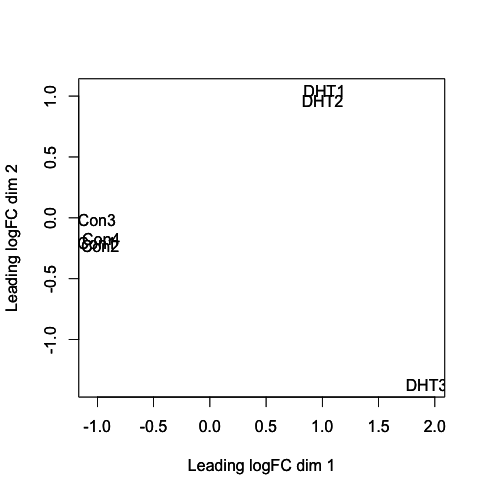
\includegraphics[width=0.8\textwidth]{handout/MDS.png}
\caption{Visualization of sample clustering}
\label{fig:MDS plot}
\end{figure}

\begin{questions}
Does the MDS plot indicate a difference in gene expression between the Controls and the DHT treated samples?\begin{answer}
The MDS plot shows us that the controls are separated from the DHT treated cells. This indicates that there is a difference in gene expression between the conditions.	
\end{answer}
\end{questions}
We will now estimate the dispersion. We start by estimating the common dispersion. The common dispersion estimates the overall Biological Coefficient of Variation (BCV) of the dataset averaged over all genes. 
\begin{steps}
By using verbose we get the Disp and BCV values printed on the screen
\begin{lstlisting}
y <- estimateCommonDisp(y, verbose=T)
\end{lstlisting}

\begin{questions}
What value to you see for BCV?
\end{questions}

\begin{steps}
We now estimate gene-specific dispersion.
\begin{lstlisting}
y <- estimateTagwiseDisp(y) 
\end{lstlisting}



We will plot the tagwise dispersion and the common dispersion (You should obtain a plot as shown in the Figure 5):
\begin{lstlisting}
plotBCV(y)
\end{lstlisting}

\end{steps}
\begin{figure}[H]
\centering
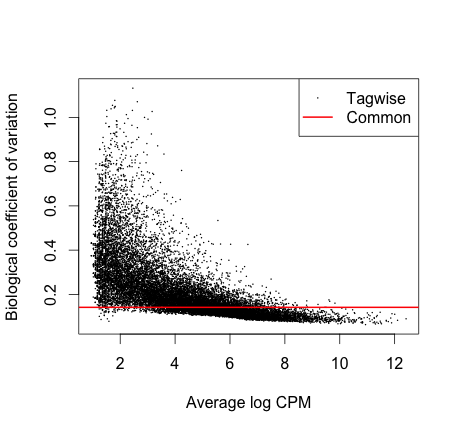
\includegraphics[width=0.8\textwidth]{handout/BCV.png}
\caption{Visualization of sample clustering}
\label{fig:BCV plot}
\end{figure}

\begin{information}
We see here that the common dispersion estimates the overall Biological Coefficient of
Variation (BCV) of the dataset averaged over all genes. The common dispersion is
\texttt{0.02} and the BCV is the square root of the common dispersion (sqrt[0.02] = 0.14).
A BCV of 14\% is typical for cell line experiment.

As you can see from the plot the BCV of some genes (generally those with low expression) can be much higher than the common dispersion. For example we see genes with a reasonable level of expression with tagwise dispersion of 0.4 indicating 40\% variation between samples. 
\end{information}


\begin{questions}
If we used the common dispersion for these genes instead of the tagwise dispersion what effect would this have?	
\end{questions}


\begin{information}
If we simply used the common dispersion for these genes we would underestimate biological variability, which in turn affects whether these genes would be identified as being differentially expressed between conditions.It is recommended to use the tagwise dispersion, which takes account of gene-to-gene variability.
	
\end{information}Now that we have normalized our data and also calculated the variability of gene expression between samples we are in a position to perform differential expression testing.As this is a simple comparison between two conditions, androgen treatment and placebo treatment we can use the exact test for the negative binomial distribution (Robinson and Smyth, 2008). 

\subsection{Testing for Differential Expression}
\begin{steps}
We now test for differentially expressed BCV genes:
\begin{lstlisting}
et <- exactTest(y)
\end{lstlisting}


Now we will use the topTags function to adjust for multiple testing. We will use the
Benjimini Hochberg ("BH") method and we will produce a table of results:
\begin{lstlisting}
res <- topTags(et, n=nrow(y$counts), adjust.method="BH")$table
\end{lstlisting}

Let's have a look at the first rows of the table:
\begin{lstlisting}
head(res)
\end{lstlisting}
\end{steps}


To get a summary of the number of differentially expressed genes we can use the decideTestsDGE function.
\begin{steps}
\begin{lstlisting}summary(de <- decideTestsDGE(et))
\end{lstlisting}
\end{steps}
This tells us that 2096 genes are downregulated and 2339 genes are upregulated at 5\% FDR.We will now make subsets of the most significant upregulated and downregulated genes.

\begin{steps}
\begin{lstlisting}
alpha=0.05
lfc=1.5
edgeR_res_sig<-res[res$FDR<alpha,]
edgeR_res_sig_lfc <-edgeR_res_sig[abs(edgeR_res_sig$logFC) >= lfc,]head(edgeR_res_sig, n=20)nrow(edgeR_res_sig)nrow(edgeR_res_sig_lfc)

\end{lstlisting}
\end{steps}
We can write out these results to our current directory.
\begin{steps}
\begin{lstlisting}
write.table(edgeR_res_sig , "edgeR_res_sig.txt", sep="\t", col.names=NA, quote=F)
write.table(edgeR_res_sig_lfc , "edgeR_res_sig_lfc.txt", sep="\t", col.names=NA, quote=F)
\end{lstlisting}

\end{steps}

\begin{questions}
How many differentially expressed genes are there? 
\begin{answer}
4435
\end{answer}

How many upregulated genes and downregulated genes do we have?
\begin{answer}
2339
2096
\end{answer}
\end{questions}

\newpage

\section{Differential expression using the Voom function and the limma package}

We will now show an alternative approach to differential expression which uses the \texttt{limma} package.This is based on linear models. The first step is to create a design matrix. In this case we have a simple design where we have only one condition (treated vs non-treated). However, you may be dealing with more complex experimental designs, for example looking at treatment and other covariates, such as age, gender, batch.

\begin{steps}
\begin{lstlisting}
design <-model.matrix(~treatment)
check design
print(design)
\end{lstlisting}
We now use voom to transform the data into a form which is appropriate for linear modelling.
\begin{lstlisting}
v <-voom(y, design)
\end{lstlisting}
\end{steps}
Next we will fit linear model to each gene in the dataset using the function lmFit.  Following this we use the function eBayes to test  each gene to find whether foldchange between the conditions being tested is statistically significant.We filter our results by using the same values of alpha (0.05) and log fold change (1.5) used previously.

\begin{steps}
\begin{lstlisting}
fit_v <-lmFit(v, design) 

fit_v <- eBayes(fit_v)

voom_res<-topTable(fit_v, coef=2,adjust.method="BH", sort.by="P", n=nrow(y$counts)) 

voom_res_sig <-voom_res[voom_res$adj.P.Val <alpha,]

voom_res_sig_lfc <-voom_res_sig[abs(voom_res_sig$logFC) >= lfc,]
\end{lstlisting}
\end{steps}

How many differentially expressed genes are identified?

\begin{steps}
\begin{lstlisting}
nrow(voom_res_sig)nrow(voom_res_sig_lfc)
\end{lstlisting}
\end{steps}
We will write out these results.

\begin{steps}
\begin{lstlisting}
write.table(voom_res_sig, "voom_res_sig.txt", sep="\t", col.names=NA, quote=F)
write.table(voom_res_sig_lfc, "voom_res_sig_lfc.txt", sep="\t", col.names=NA, quote=F)
write.table(voom_res, "voom_res.txt", sep="\t", col.names=NA, quote=F) 
\end{lstlisting}
\end{steps}

\section{Data Visualisation}
Now let's visualize some of this data. First we will make a volcano plot using the \texttt{volcanoplot} function available in \texttt{limma}. This creates a plot which displays fold changes versus a measure of statistical significance of the change.

\begin{steps}
\begin{lstlisting}
volcanoplot(fit_v, coef=2, highlight=5)
\end{lstlisting}
\end{steps}

\begin{figure}[H]
\centering
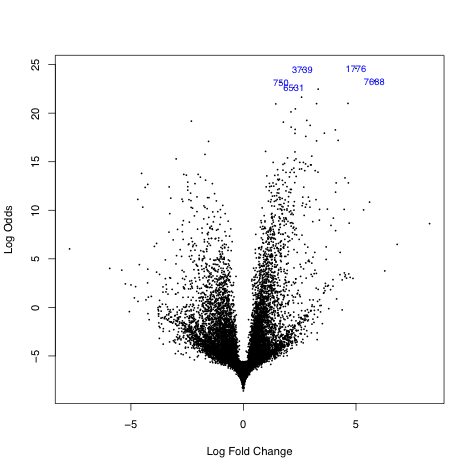
\includegraphics[width=0.8\textwidth]{handout/Volcano.png}
\caption{Volcano Plot}
\label{fig:Volcano plot}
\end{figure}

Next we will create a heatmap of the top differentially expressed genes. We use the heatmap.2 function available in the gplots package.
\begin{steps}
\begin{lstlisting}
select_top  <- p.adjust(fit_v$p.value[, 2]) <1e-2
Exp_top <- v$E [select_top, ]
heatmap.2(Exp_top, scale="row", density.info="none", trace="none", main="Top DEGs", labRow="", cexRow=0.4, cexCol=0.8)
\end{lstlisting}
\end{steps}

\begin{figure}[H]
\centering
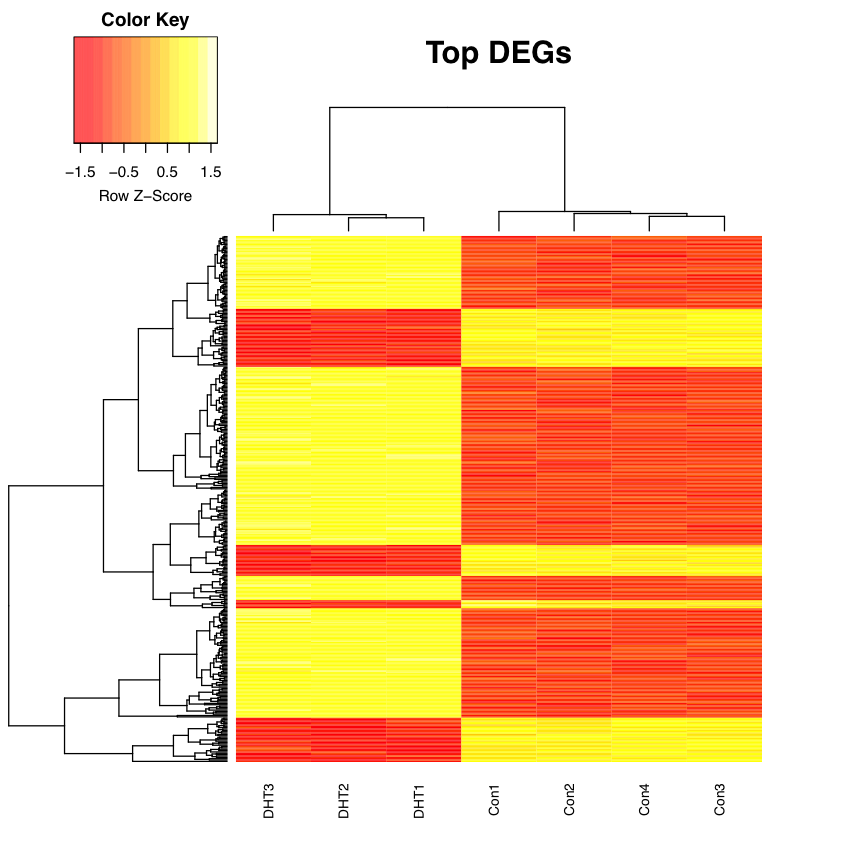
\includegraphics[width=0.8\textwidth]{handout/Heatmap.png}
\caption{Heatmap of DE genes}
\label{fig:Heatmap}
\end{figure}


% END of the R SESSION
You can now quit the R prompt
\begin{lstlisting}
q()
\end{lstlisting}
\end{steps}
You can save your workspace by typing \texttt{Y} on prompt.
\begin{note}
Please note that the output files you are creating are saved in your present working directory. If you are not sure where you are in the file system try typing \texttt{pwd} on your command prompt to find out.
\end{note}

% Bonus cufflinks: This will be run only for the longer workshops. Skip for 2day format. Users can try the commands at home.

\begin{bonus}

\section{Differential Expression using cuffdiff}

\begin{warning}
This is optional exercise and will be run if time permits. 
\end{warning}

One of the stand-alone tools that perform differential expression analysis is
Cuffdiff. We use this tool to compare between two conditions; for example
different conditions could be control and disease, or wild-type and mutant, or
various developmental stages.

In our case we want to identify genes that are differentially expressed between
two developmental stages; a \texttt{2cells} embryo and \texttt{6h} post
fertilization.

\begin{information}
The general format of the cuffdiff command is:

\begin{lstlisting}[style=command_syntax]
cuffdiff [options]* <transcripts.gtf> <sample1_replicate1.sam[,...,sample1_replicateM]> <sample2_replicate1.sam[,...,sample2_replicateM.sam]>
\end{lstlisting}

Where the input includes a \texttt{transcripts.gtf} file, which is an annotation
file of the genome of interest or the cufflinks assembled transcripts, and the aligned reads (either in SAM or BAM
format) for the conditions.
Some of the Cufflinks options that we will use to run the program are:

\begin{description}[style=multiline,labelindent=0cm,align=right,leftmargin=\descriptionlabelspace,rightmargin=1.5cm,font=\ttfamily]
  \item[-o] Output directory.
  \item[-L] Labels for the different conditions
  \item[-T] Tells Cuffdiff that the reads are from a time series experiment.
  \item[-b] Instructs Cufflinks to run a bias detection and correction algorithm
  which can significantly improve accuracy of transcript abundance estimates.
  To do this Cufflinks requires a multi-fasta file with the genomic sequences
  against which we have aligned the reads.
  \item[-u] Tells Cufflinks to do an initial estimation procedure to more
  accurately weight reads mapping to multiple locations in the genome
  (multi-hits). 
  \item[--library-type] Before performing any type of RNA-seq analysis you need
 to know a few things about the library preparation. Was it done using a
 strand-specific protocol or not? If yes, which strand? In our data the protocol
 was NOT strand specific.
  \item[-C] Biological replicates and multiple group contrast can be defined here 
\end{description}

\end{information}

\begin{steps}
Run cuffdiff on the tophat generated BAM files for the 2cells vs. 6h data sets:
\begin{lstlisting}
cuffdiff -o cuffdiff/ -L ZV9_2cells,ZV9_6h -T -b genome/Danio_rerio.Zv9.66.dna.fa -u --library-type fr-unstranded annotation/Danio_rerio.Zv9.66.gtf tophat/ZV9_2cells/accepted_hits.bam tophat/ZV9_6h/accepted_hits.bam
\end{lstlisting}
\end{steps}

\begin{steps}
We are interested in the differential expression at the gene level. The results
are reported by Cuffdiff in the file \texttt{cuffdiff/gene\_exp.diff}. 
Look at the first few lines of the file using the following command:
\begin{lstlisting}
head -n 20 cuffdiff/gene_exp.diff
\end{lstlisting}

We would like to see which are the most significantly differentially expressed
genes. Therefore we will sort the above file according to the q value
(corrected p value for multiple testing). The result will be stored in a
different file called \texttt{gene\_exp\_qval.sorted.diff}.
\begin{lstlisting}
sort -t$'\t' -g -k 13 cuffdiff/gene_exp.diff > cuffdiff/gene_exp_qval.sorted.diff
\end{lstlisting}

Look again at the top 20 lines of the sorted file by typing:
\begin{lstlisting}
head -n 20 cuffdiff/gene_exp_qval.sorted.diff
\end{lstlisting}
Copy an Ensembl transcript identifier from the first two columns for one of
these genes (e.g. \texttt{ENSDARG00000045067}). Now go back to the IGV browser
and paste it in the search box.
\end{steps}

\begin{questions}
What are the various outputs generated by cuffdiff?
Hint: Please refer to the \texttt{Cuffdiff output} section of the cufflinks manual online.

Do you see any difference in the read coverage between the \texttt{2cells} and
\texttt{6h} conditions that might have given rise to this transcript being
called as differentially expressed?
\begin{warning}
The coverage on the Ensembl browser is based on raw reads and no
normalisation has taken place contrary to the FPKM values.
\end{warning}

\begin{answer}
The read coverage of this transcript (\texttt{ENSDARG00000045067}) in the 6h
data set is much higher than in the 2cells data set.
\end{answer}
\end{questions}


\section{Visualising the CuffDiff expression analysis}
We will use an R-Bioconductor package called \texttt{cummeRbund} to visualise, manipulate and explore Cufflinks RNA-seq output. We will load an R environment and look at few quick tips to generate simple graphical output of the cufflinks analysis we have just run.

\begin{information}
\texttt{CummeRbund} takes the cuffdiff output and populates a SQLite database with various type of output generated by cuffdiff e.g, genes, transcripts, transcription start site, isoforms and CDS regions. The data from this database can be accessed and processed easily. This package comes with a number of in-built plotting functions that are commonly used for visualising the expression data. We strongly recommend reading through the bioconductor manual and user guide of CummeRbund to learn about functionality of the tool. The reference is provided in the resource section.
\end{information}

\begin{steps}
Prepare the environment. Go to the \texttt{cuffdiff} output folder and copy the transcripts file there.
\begin{lstlisting}
cd ~/rnaseq/cuffdiff
cp ~/rnaseq/annotation/Danio_rerio.Zv9.66.gtf ~/rnaseq/cuffdiff
ls -l
\end{lstlisting}

Load the R environment
\begin{lstlisting}
R (press enter)
\end{lstlisting}
Load the require R package.
\begin{lstlisting}
library(cummeRbund)
\end{lstlisting}
Read in the cuffdiff output
\begin{lstlisting}
cuff<-readCufflinks(dir="/home/trainee/Desktop/rnaseq/cuffdiff", \
gtfFile='Danio_rerio.Zv9.66.gtf',genome="Zv9", rebuild=T)
\end{lstlisting}
Assess the distribution of FPKM scores across samples
\begin{lstlisting}
pdf(file = "SCV.pdf", height = 6, width = 6)
dens<-csDensity(genes(cuff))
dens
dev.off()
\end{lstlisting}
Box plots of the FPKM values for each samples
\begin{lstlisting}
pdf(file = "BoxP.pdf", height = 6, width = 6)
b<-csBoxplot(genes(cuff))
b
dev.off()
\end{lstlisting}



Accessing the data
\begin{lstlisting}
sigGeneIds<-getSig(cuff,alpha=0.05,level="genes")
head(sigGeneIds)
sigGenes<-getGenes(cuff,sigGeneIds)
sigGenes
head(fpkm(sigGenes))
head(fpkm(isoforms(sigGenes)))
\end{lstlisting}
Plotting a heatmap of the differentially expressed genes
\begin{lstlisting}
pdf(file = "heatmap.pdf", height = 6, width = 6)
h<-csHeatmap(sigGenes,cluster="both")
h
dev.off()
\end{lstlisting}
\end{steps}

\begin{questions}
What options would you use to draw a density or boxplot for different replicates if available ? 
(Hint: look at the manual at Bioconductor website)
\begin{answer}
\begin{lstlisting}
densRep<-csDensity(genes(cuff),replicates=T)
brep<-csBoxplot(genes(cuff),replicates=T)
\end{lstlisting}
\end{answer}
\end{questions}

\begin{questions}
How many differentially expressed genes did you observe?

\begin{answer}
type 'summary(sigGenes)' on the R prompt to see.
\end{answer}
\end{questions}

\end{bonus}

\newpage

\section{References}
\begin{enumerate}
  \item Trapnell, C., Pachter, L. \& Salzberg, S. L. TopHat: discovering splice
  junctions with RNA-Seq. Bioinformatics 25, 1105-1111 (2009).
  \item Trapnell, C. et al. Transcript assembly and quantification by RNA-Seq
  reveals unannotated transcripts and isoform switching during cell
  differentiation. Nat. Biotechnol. 28, 511-515 (2010).
  \item Langmead, B., Trapnell, C., Pop, M. \& Salzberg, S. L. Ultrafast and
  memory-efficient alignment of short DNA sequences to the human genome.
  Genome Biol. 10, R25 (2009).
  \item Roberts, A., Pimentel, H., Trapnell, C. \& Pachter, L. Identification
  of novel transcripts in annotated genomes using RNA-Seq. Bioinformatics 27,
  2325-2329 (2011).
  \item Roberts, A., Trapnell, C., Donaghey, J., Rinn, J. L. \& Pachter, L.
  Improving RNA-Seq expression estimates by correcting for fragment bias.
  Genome Biol. 12, R22 (2011).
  \item Robinson MD, McCarthy DJ and Smyth GK. edgeR: a Bioconductor package for 
  differential expression analysis of digital gene expression data.
  Bioinformatics, 26 (2010).
  \item Robinson MD and Smyth GK Moderated statistical tests for assessing 
  differences in tag abundance. Bioinformatics, 23, pp. -6.
  \item Robinson MD and Smyth GK (2008). Small-sample estimation of negative 
  binomial dispersion, with applications to SAGE data.” Biostatistics, 9.
  \item McCarthy, J. D, Chen, Yunshun, Smyth and K. G (2012). Differential 
  expression analysis of multifactor RNA-Seq experiments with respect to 
  biological variation. Nucleic Acids Research, 40(10), pp. -9.
\end{enumerate}
